% This document is used for Daya Bay MACRO PMT pressure test report


\documentclass{beamer}
\usepackage{graphicx}

\newcommand{\tabincell}[2]{\begin{tabular}{@{}#1@{}}#2\end{tabular}}

\usepackage{ragged2e}
\justifying

\usepackage{setspace}

\setbeamertemplate{navigation symbols}{}
\setbeamertemplate{footline}[page number]
\setbeamertemplate{caption}[numbered]

\usetheme{default}
\logo{
\includegraphics[height=1cm]{Dyb_logo.png}}
\begin{document}
\title{Status of MACRO \& Hamamatsu PMT pressure tests at SAB}
\author{Logan Lebanowski, Shih-Kai Lin}
\institute{University of Houston}
\date{2010 October 21}

\begin{frame}
\begin{center}
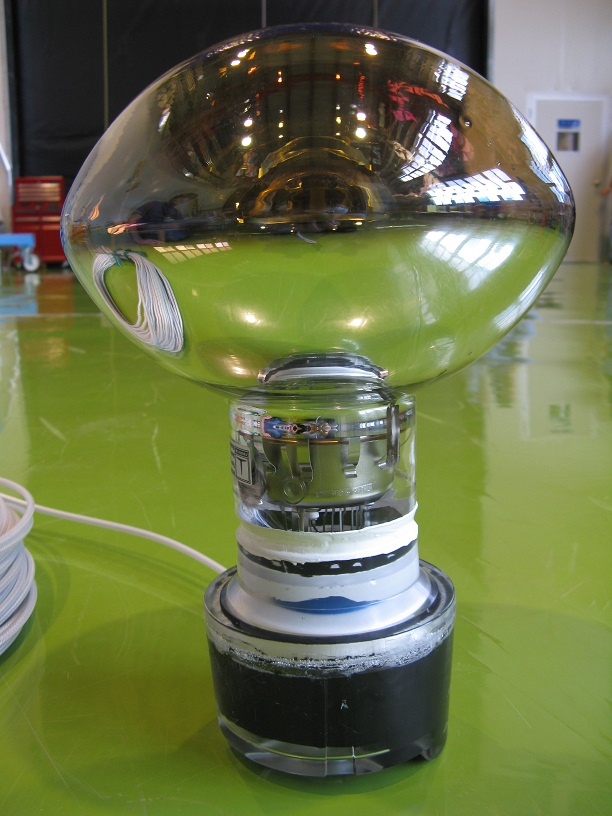
\includegraphics[height=4cm]{IMG_1048.jpg}
\end{center}
\titlepage
\end{frame}


\begin{frame}{overview}
	\begin{itemize}
		\item 150 waterproof MACRO EMI PMT assemblies as well as 16
			Hamamatsu waterproof PMTs need to be pressure tested
			at the SAB. They have already passed performance tests at DGUT.
		\item We test about 10 PMTs per week (mid-August to December).
		\item For more information, see
			\textcolor{blue}{\href
			{http://dayabay.ihep.ac.cn/cgi-bin/DocDB/ShowDocument?docid=5373}{doc 5373}}.
	\end{itemize}
		\begin{center}
			\underline{As of October 21, we have passed 71 of 79 tested MACRO PMTs}\\
			\underline{and 6 of 6 tested Hamamatsu PMTs.}
		\end{center}
	\begin{center}
		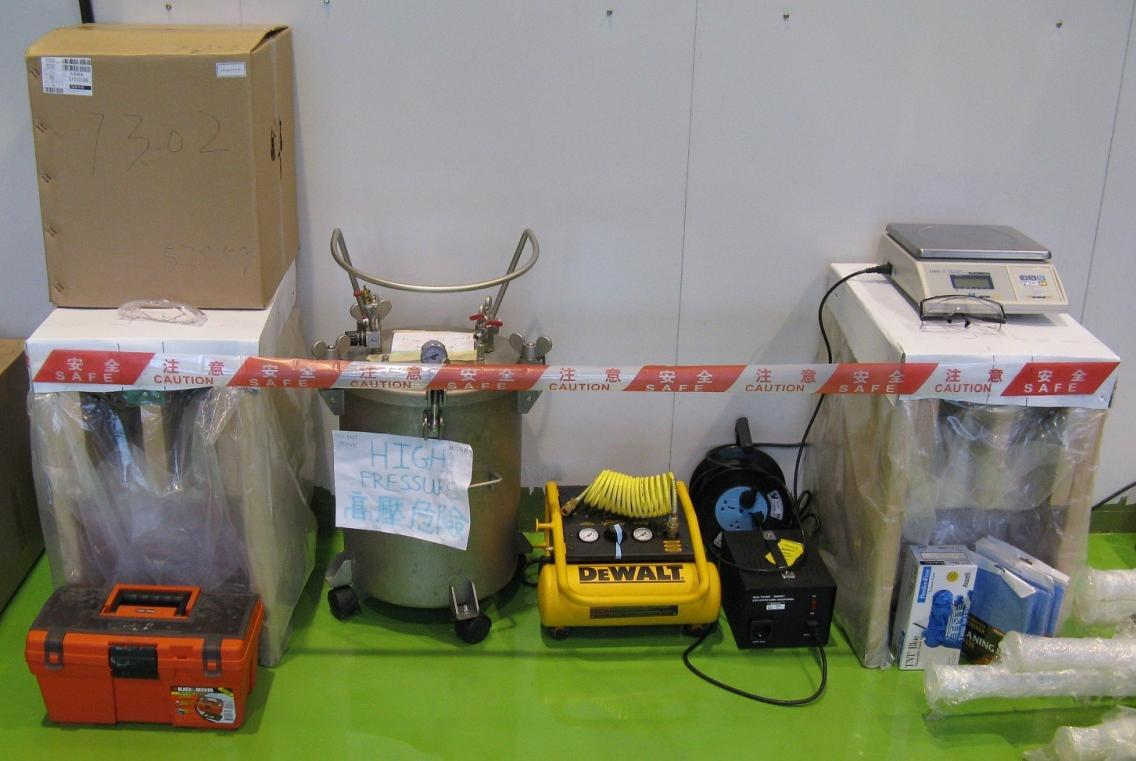
\includegraphics[height=4cm]{test_setup.jpeg}
	\end{center}
\end{frame}


\begin{frame}{pressure test results}
	\begin{center}
		\small
		6 PMTs were tested during the past week (October 14 - October 20).
	\end{center}
\begin{table}
\small
\setstretch{0.4}
\begin{tabular}{|c|c|c|c|c|}
%\setlength{\tabcolsep}{2pt}
	\hline
	SN$^\dagger$ & mass$^\ddag$(g) & pressure (psig) & test time (h:m) & result \\
	\hline
	WSD2720 & 4601.0 & 14.1 & 14:57 & PASS$^1$ \\
	\hline
	8170 & 547.0 & 12.4 & 8:11 & PASS$^2$ \\
	\hline
	WSD2597 & 4594.0 & 14.3 & 15:24 & PASS$^1$ \\
	\hline
	WSD2653 & 4600.5.0 & 14.3 & 23:17 & PASS$^1$ \\
	\hline
	WSD2721 & 4612.0 & 14.1 & 76:57 & PASS$^1$ \\
	\hline
	WSD2657 & 4422.0 & 14.3 & 22:35 & PASS$^1$ \\
	\hline
\end{tabular}
%\caption {pressure test result: For PASS/FAIL reasons, please see the table in the next slide.}
\end{table}
	\setstretch{0.1}
	\scriptsize
	$^\dagger$ Serinal numbers with ``WSD'' prefix are Hamamatsu waterproof PMTs. \\
	$^\ddag$ For MACRO PMTs, this means unpotted weight. For Hamamatsu PMTs, this is the total
			weight of PMT+cable.
%\begin{itemize}
%	\item For PASS/FAIL reasons, please see the table in the next slide.
%\end{itemize}
	\setlength{\tabcolsep}{2pt}
	\scriptsize
	\begin{table}
		\begin{tabular}{|c|p{3.5in}|}
		\hline
		1 & Cable dry. No cracks. No leaks detected to within 2.0g
		    (determined by weighing before and after testing.)\\
		\hline
		2 & Cable dry. No leaks or cracks. \\
		\hline
%		3 & Cable sealing tube still had some water. The way the cable was repaired didn't
%		work well.\\
%		\hline
		\end{tabular}
	%\caption{PASS/FAIL reasons}
	\end{table}
\end{frame}


\begin{frame}{signal test results}
	\setstretch{0.3}
	\small The operational capability of a PMT is verified after pressure testing:\\
	{\scriptsize The PMT is placed in a dark box, connected to a single channel decoupler box,
	and set to its 2E7 gain voltage, as recorded in the DGUT data. After tens of minutes,
	the count rate, rise time, and pulse height are recorded. We use a threshold of 3.00 
	mV, which is roughly 1/4 pe.
	}

	\setstretch{1}
	\setlength{\tabcolsep}{2pt}
	\small
	\begin{center}
		\begin{itemize}
			\item Due to installation workshop, no signal tests were done this week. Since 
			we have the HV datasheet for Hamamatsu waterproof PMTs, we will signal test them
			next week.
		\end{itemize}

	\end{center}
\end{frame}


\end{document}

